\section{Grundglieder}
\subsection{Statische Glieder}
Bei einem statische Glied ist der aktuelle Wert des Ausgangssignal $y$ nur vom aktuelle Wert des Eingangssignal $u$ abhängig:
\[y = f(u)\]
Beispiele:
\begin{center}
	\begin{minipage}{0.10\textwidth}
		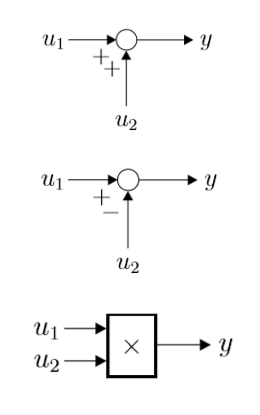
\includegraphics[width=\linewidth,keepaspectratio=true]{Images/statischeglieder}
	\end{minipage}%%% to prevent a space
	\begin{minipage}{0.3\textwidth}
		\[y = u_1 + u_2 \]
		\[y = u_1 - u_2 \]
		\[y = u_1 \cdot u_2 \]
	\end{minipage}
\end{center}

\subsubsection{Proportionalglied (P-Glied)}
Für ein P-Glied gilt der proportionale Zusammenhang:

\begin{center}
	\begin{minipage}{0.10\textwidth}
		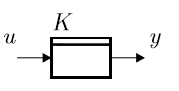
\includegraphics[width=\linewidth,keepaspectratio=true]{Images/pglied}
	\end{minipage}%%% to prevent a space
	\begin{minipage}{0.3\textwidth}
		\[y = K \cdot u\]
	\end{minipage}
\end{center}


\subsubsection{Integrierer (I-Glied)}
Gegenüber statischen gelidern hat ein dynamisches I-Glied einen Zustandsspeicher und ist abhängig von vorhergehenden Zuständen:

\begin{center}
	\begin{minipage}{0.10\textwidth}
		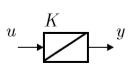
\includegraphics[width=\linewidth,keepaspectratio=true]{Images/iglied}
	\end{minipage}%%% to prevent a space
	\begin{minipage}{0.3\textwidth}
		\begin{align*}
			y(t) &= K \cdot \int_{\tau=0}^{t}u(\tau)d\tau + y(0) \\
			\dot{y}(t) &= K \cdot u(t)
		\end{align*}
	\end{minipage}
\end{center}

\subsubsection{idealer Differenzierer (D-Glied)}
Idealer Differenzierer funktioniert idealerweise umgekehrt wie der Integrator (I-Glied). Ebenfalls mit einem Verstärkungsfaktor $K$.

\begin{center}
	\begin{minipage}{0.10\textwidth}
		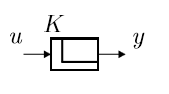
\includegraphics[width=\linewidth,keepaspectratio=true]{Images/dglied}
	\end{minipage}%%% to prevent a space
	\begin{minipage}{0.3\textwidth}
		\begin{align*}
			y(t) &= K \cdot \frac{du}{dt}(t) = K\cdot \dot{u}(t)
		\end{align*}
	\end{minipage}
\end{center}


\subsubsection{Totzeit Glied}
Bei einem Totzeitglied erscheint das Eingangssignal um die Totzeit $T_t$ verzögert am Ausgang.

\begin{center}
	\begin{minipage}{0.10\textwidth}
		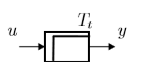
\includegraphics[width=\linewidth,keepaspectratio=true]{Images/totzeitglied}
	\end{minipage}%%% to prevent a space
	\begin{minipage}{0.3\textwidth}
		\begin{align*}
			y(t) &= u(t - T_t)
		\end{align*}
	\end{minipage}
\end{center}

\subsubsection{PT$_1$ Glied}\script{31}
Das PT$_1$-Glied hat eine Verstärkungsfaktor $K$ mit Verzögerung $T$. Falls $T=0$ ergibt sich wieder ein P-Glied.
\begin{center}
	\begin{minipage}{0.20\textwidth}
		\begin{center}
			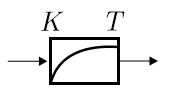
\includegraphics[width=0.5\linewidth,keepaspectratio=true]{Images/pt1glied}\\
			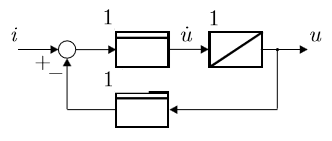
\includegraphics[width=\columnwidth]{Images/pt1glied_adv}
		\end{center}
	\end{minipage}%%% to prevent a space
	\begin{minipage}{0.3\textwidth}
		\begin{align*}
			T \cdot \dot{y}(t) + y(t) = K \cdot u(t)
		\end{align*}
		Mit der DGL-Lösung ($u(t) = A \cdot \varepsilon(t)$)
		\begin{align*}
			y(t) &= KA +(y_0 - KA)\cdot e^{-\frac{t}{T}}\\ 
			\xrightarrow{y_0 = 0} y(t) &= KA (1 -e^{-\frac{t}{T}}) \\ 
		\end{align*}
	\end{minipage}
\end{center}


Hilfegrössen können bei einem PT$_1$ \textbf{grafisch Ausgemessen} oder Berechnet werden. Das Grafische Ausmessen von $T$ kann durch anlegen einer Tangente am Ursprung und dem Schnittpunkt der $KA$ Asymptote bei $~63\%$ mit Messen der x-Achse erfolgen. Der Parameter $K = \frac{y_\infty}{A}$ ergibt sich durch rechnnen.
\begin{center}
	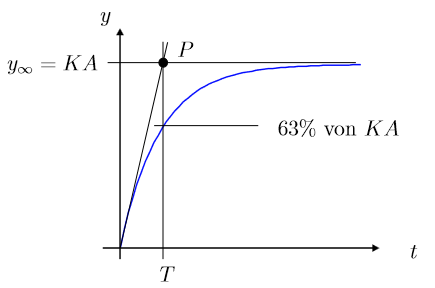
\includegraphics[width=0.6\columnwidth]{Images/pt1_graph}
\end{center}

\subsubsection{PT$_2$ Glied}\script{34}
Das PT$_2$-Glied hat einen Verstärkungsfaktor $K$ (verändern der y-Achse), Zeitkonstante $T$ (verändern der x-Achse) und Dämpfkonstante $\zeta$.

\begin{center}
	\begin{minipage}{0.20\textwidth}
		\begin{center}
			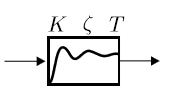
\includegraphics[width=0.5\linewidth,keepaspectratio=true]{Images/pt2glied}\\
		\end{center}
	\end{minipage}%%% to prevent a space
	\begin{minipage}{0.3\textwidth}
		\begin{align*}
			T^2 \cdot \ddot{y}(t) + 2\zeta T \cdot \dot{y}(t) + y(t) = K \cdot u(t)
		\end{align*}
		DGL lösen mit Char.Polynom.
	\end{minipage}
\end{center}

PT$_2$ Hilfsgrössen können bei einem System ausgerechnet werden:
\begin{align*}
	h &= \log\left(\frac{y_m}{y_\infty}\right) ;\quad \omega = \frac{\pi}{T_m} = \frac{2\pi}{T_\omega} ;\quad \sigma = \frac{h\omega}{\pi}\\
	K &= \frac{y_\infty}{A}\\
	\zeta &= \frac{h}{\sqrt{h^2 + \pi^2}}\\
	T &= \frac{1}{\sqrt{\omega^2 + \sigma^2}}
\end{align*}
\begin{center}
	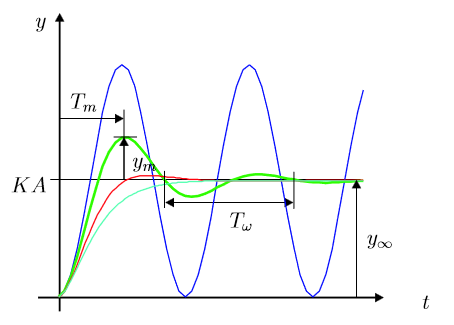
\includegraphics[width=0.6\columnwidth]{Images/pt2_graph}
\end{center}


\subsubsection{Sättigungsglied}
\begin{center}
	\begin{minipage}{0.20\textwidth}
		\begin{center}
			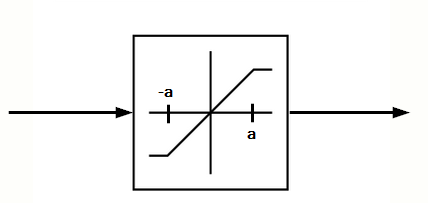
\includegraphics[width=0.5\linewidth,keepaspectratio=true]{Images/saturationglied}\\
		\end{center}
	\end{minipage}%%% to prevent a space
	\begin{minipage}{0.3\textwidth}
		\begin{align*}
			y(t) = 	\begin{cases}
				u_{max} & \text{Wenn } u(t) \ge a\\
				u(t) & \text{sonst } \\
				u_{min} & \text{Wenn }  u(t) \le -a
			\end{cases}
		\end{align*}
	\end{minipage}
\end{center}

